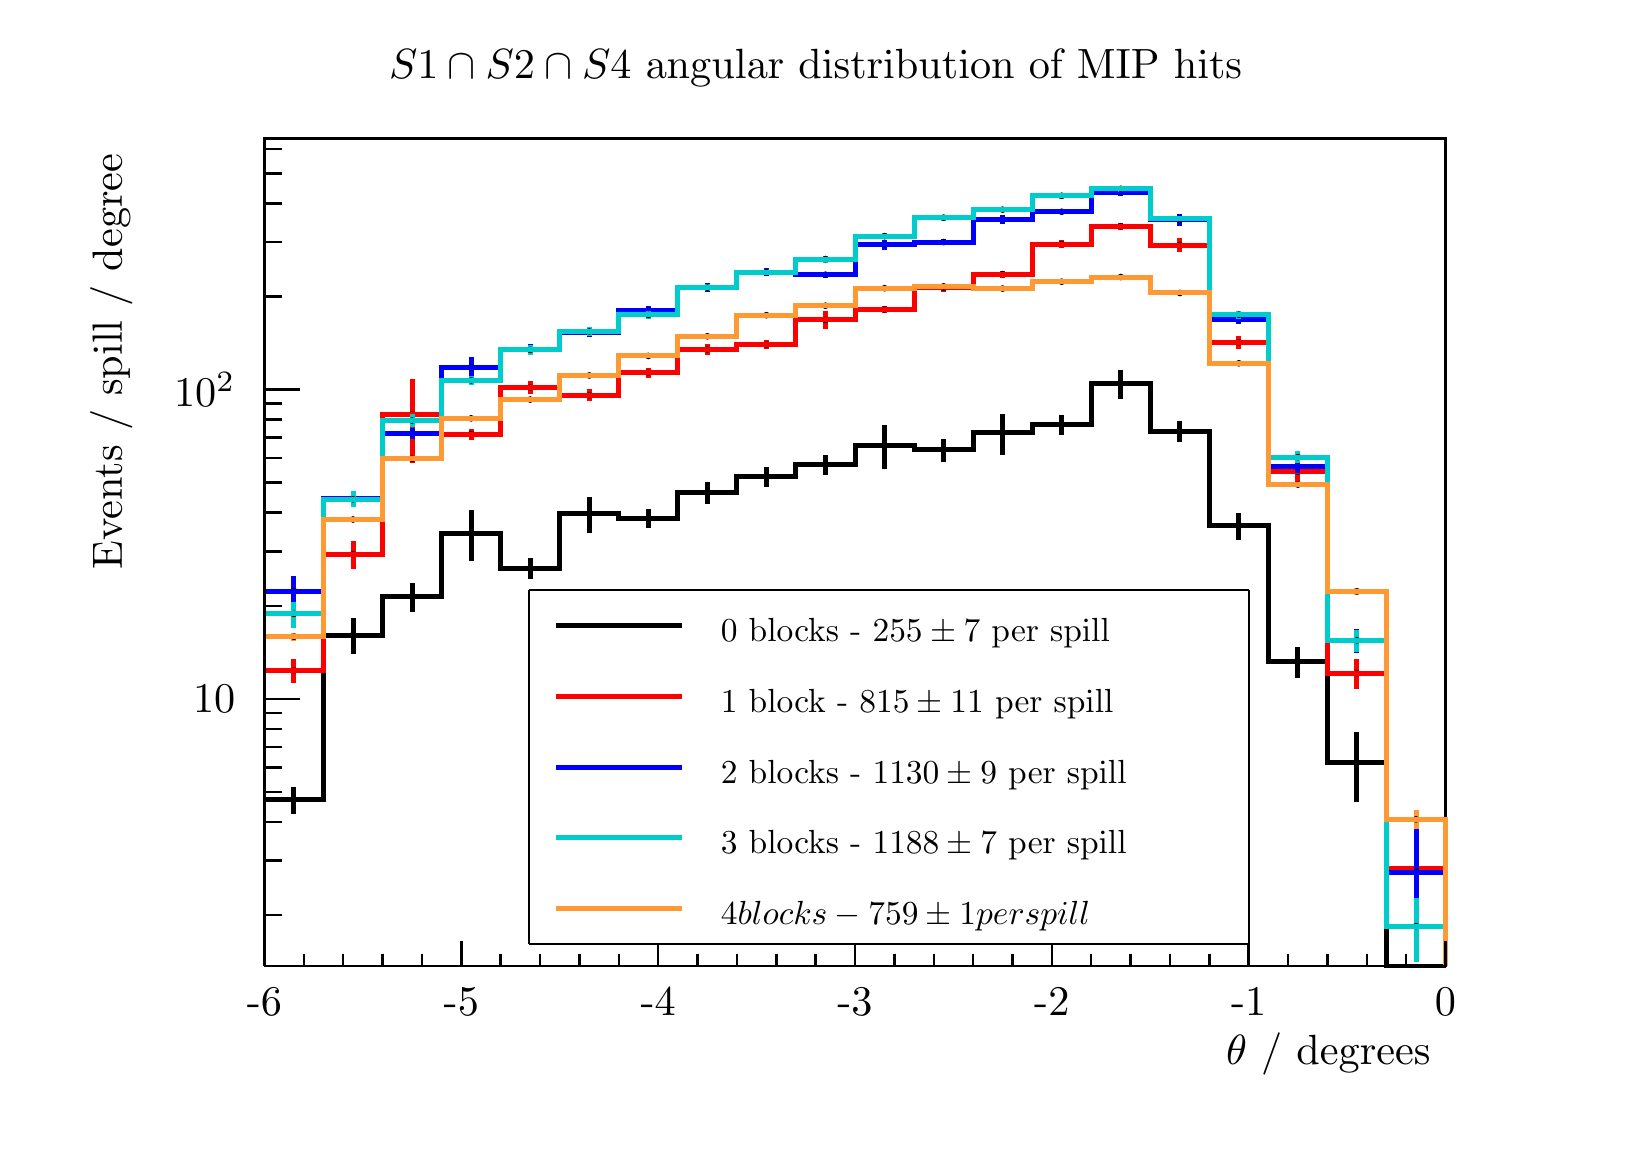
\begin{tikzpicture}
\pgfdeclareplotmark{cross} {
\pgfpathmoveto{\pgfpoint{-0.3\pgfplotmarksize}{\pgfplotmarksize}}
\pgfpathlineto{\pgfpoint{+0.3\pgfplotmarksize}{\pgfplotmarksize}}
\pgfpathlineto{\pgfpoint{+0.3\pgfplotmarksize}{0.3\pgfplotmarksize}}
\pgfpathlineto{\pgfpoint{+1\pgfplotmarksize}{0.3\pgfplotmarksize}}
\pgfpathlineto{\pgfpoint{+1\pgfplotmarksize}{-0.3\pgfplotmarksize}}
\pgfpathlineto{\pgfpoint{+0.3\pgfplotmarksize}{-0.3\pgfplotmarksize}}
\pgfpathlineto{\pgfpoint{+0.3\pgfplotmarksize}{-1.\pgfplotmarksize}}
\pgfpathlineto{\pgfpoint{-0.3\pgfplotmarksize}{-1.\pgfplotmarksize}}
\pgfpathlineto{\pgfpoint{-0.3\pgfplotmarksize}{-0.3\pgfplotmarksize}}
\pgfpathlineto{\pgfpoint{-1.\pgfplotmarksize}{-0.3\pgfplotmarksize}}
\pgfpathlineto{\pgfpoint{-1.\pgfplotmarksize}{0.3\pgfplotmarksize}}
\pgfpathlineto{\pgfpoint{-0.3\pgfplotmarksize}{0.3\pgfplotmarksize}}
\pgfpathclose
\pgfusepathqstroke
}
\pgfdeclareplotmark{cross*} {
\pgfpathmoveto{\pgfpoint{-0.3\pgfplotmarksize}{\pgfplotmarksize}}
\pgfpathlineto{\pgfpoint{+0.3\pgfplotmarksize}{\pgfplotmarksize}}
\pgfpathlineto{\pgfpoint{+0.3\pgfplotmarksize}{0.3\pgfplotmarksize}}
\pgfpathlineto{\pgfpoint{+1\pgfplotmarksize}{0.3\pgfplotmarksize}}
\pgfpathlineto{\pgfpoint{+1\pgfplotmarksize}{-0.3\pgfplotmarksize}}
\pgfpathlineto{\pgfpoint{+0.3\pgfplotmarksize}{-0.3\pgfplotmarksize}}
\pgfpathlineto{\pgfpoint{+0.3\pgfplotmarksize}{-1.\pgfplotmarksize}}
\pgfpathlineto{\pgfpoint{-0.3\pgfplotmarksize}{-1.\pgfplotmarksize}}
\pgfpathlineto{\pgfpoint{-0.3\pgfplotmarksize}{-0.3\pgfplotmarksize}}
\pgfpathlineto{\pgfpoint{-1.\pgfplotmarksize}{-0.3\pgfplotmarksize}}
\pgfpathlineto{\pgfpoint{-1.\pgfplotmarksize}{0.3\pgfplotmarksize}}
\pgfpathlineto{\pgfpoint{-0.3\pgfplotmarksize}{0.3\pgfplotmarksize}}
\pgfpathclose
\pgfusepathqfillstroke
}
\pgfdeclareplotmark{newstar} {
\pgfpathmoveto{\pgfqpoint{0pt}{\pgfplotmarksize}}
\pgfpathlineto{\pgfqpointpolar{44}{0.5\pgfplotmarksize}}
\pgfpathlineto{\pgfqpointpolar{18}{\pgfplotmarksize}}
\pgfpathlineto{\pgfqpointpolar{-20}{0.5\pgfplotmarksize}}
\pgfpathlineto{\pgfqpointpolar{-54}{\pgfplotmarksize}}
\pgfpathlineto{\pgfqpointpolar{-90}{0.5\pgfplotmarksize}}
\pgfpathlineto{\pgfqpointpolar{234}{\pgfplotmarksize}}
\pgfpathlineto{\pgfqpointpolar{198}{0.5\pgfplotmarksize}}
\pgfpathlineto{\pgfqpointpolar{162}{\pgfplotmarksize}}
\pgfpathlineto{\pgfqpointpolar{134}{0.5\pgfplotmarksize}}
\pgfpathclose
\pgfusepathqstroke
}
\pgfdeclareplotmark{newstar*} {
\pgfpathmoveto{\pgfqpoint{0pt}{\pgfplotmarksize}}
\pgfpathlineto{\pgfqpointpolar{44}{0.5\pgfplotmarksize}}
\pgfpathlineto{\pgfqpointpolar{18}{\pgfplotmarksize}}
\pgfpathlineto{\pgfqpointpolar{-20}{0.5\pgfplotmarksize}}
\pgfpathlineto{\pgfqpointpolar{-54}{\pgfplotmarksize}}
\pgfpathlineto{\pgfqpointpolar{-90}{0.5\pgfplotmarksize}}
\pgfpathlineto{\pgfqpointpolar{234}{\pgfplotmarksize}}
\pgfpathlineto{\pgfqpointpolar{198}{0.5\pgfplotmarksize}}
\pgfpathlineto{\pgfqpointpolar{162}{\pgfplotmarksize}}
\pgfpathlineto{\pgfqpointpolar{134}{0.5\pgfplotmarksize}}
\pgfpathclose
\pgfusepathqfillstroke
}
\definecolor{c}{rgb}{1,1,1};
\draw [color=c, fill=c] (0,0) rectangle (20,14.0115);
\draw [color=c, fill=c] (3,2.10172) rectangle (18,12.6103);
\definecolor{c}{rgb}{0,0,0};
\draw [c,line width=0.9] (3,2.10172) -- (3,12.6103) -- (18,12.6103) -- (18,2.10172) -- (3,2.10172);
\definecolor{c}{rgb}{1,1,1};
\draw [color=c, fill=c] (3,2.10172) rectangle (18,12.6103);
\definecolor{c}{rgb}{0,0,0};
\draw [c,line width=0.9] (3,2.10172) -- (3,12.6103) -- (18,12.6103) -- (18,2.10172) -- (3,2.10172);
\definecolor{c}{rgb}{0,0,0.6};
\draw [c,line width=0.9] (3,2.10172) -- (3.75,2.10172) -- (3.75,2.10172) -- (4.5,2.10172) -- (4.5,2.10172) -- (5.25,2.10172) -- (5.25,2.10172) -- (6,2.10172) -- (6,2.10172) -- (6.75,2.10172) -- (6.75,2.10172) -- (7.5,2.10172) -- (7.5,2.10172) --
 (8.25,2.10172) -- (8.25,2.10172) -- (9,2.10172) -- (9,2.10172) -- (9.75,2.10172) -- (9.75,2.10172) -- (10.5,2.10172) -- (10.5,2.10172) -- (11.25,2.10172) -- (11.25,2.10172) -- (12,2.10172) -- (12,2.10172) -- (12.75,2.10172) -- (12.75,2.10172) --
 (13.5,2.10172) -- (13.5,2.10172) -- (14.25,2.10172) -- (14.25,2.10172) -- (15,2.10172) -- (15,2.10172) -- (15.75,2.10172) -- (15.75,2.10172) -- (16.5,2.10172) -- (16.5,2.10172) -- (17.25,2.10172) -- (17.25,2.10172) -- (18,2.10172) -- (18,2.10172);
\definecolor{c}{rgb}{0,0,0};
\draw [c,line width=0.9] (3,2.10172) -- (18,2.10172);
\draw [c,line width=0.9] (3,2.41698) -- (3,2.10172);
\draw [c,line width=0.9] (3.5,2.25935) -- (3.5,2.10172);
\draw [c,line width=0.9] (4,2.25935) -- (4,2.10172);
\draw [c,line width=0.9] (4.5,2.25935) -- (4.5,2.10172);
\draw [c,line width=0.9] (5,2.25935) -- (5,2.10172);
\draw [c,line width=0.9] (5.5,2.41698) -- (5.5,2.10172);
\draw [c,line width=0.9] (6,2.25935) -- (6,2.10172);
\draw [c,line width=0.9] (6.5,2.25935) -- (6.5,2.10172);
\draw [c,line width=0.9] (7,2.25935) -- (7,2.10172);
\draw [c,line width=0.9] (7.5,2.25935) -- (7.5,2.10172);
\draw [c,line width=0.9] (8,2.41698) -- (8,2.10172);
\draw [c,line width=0.9] (8.5,2.25935) -- (8.5,2.10172);
\draw [c,line width=0.9] (9,2.25935) -- (9,2.10172);
\draw [c,line width=0.9] (9.5,2.25935) -- (9.5,2.10172);
\draw [c,line width=0.9] (10,2.25935) -- (10,2.10172);
\draw [c,line width=0.9] (10.5,2.41698) -- (10.5,2.10172);
\draw [c,line width=0.9] (11,2.25935) -- (11,2.10172);
\draw [c,line width=0.9] (11.5,2.25935) -- (11.5,2.10172);
\draw [c,line width=0.9] (12,2.25935) -- (12,2.10172);
\draw [c,line width=0.9] (12.5,2.25935) -- (12.5,2.10172);
\draw [c,line width=0.9] (13,2.41698) -- (13,2.10172);
\draw [c,line width=0.9] (13.5,2.25935) -- (13.5,2.10172);
\draw [c,line width=0.9] (14,2.25935) -- (14,2.10172);
\draw [c,line width=0.9] (14.5,2.25935) -- (14.5,2.10172);
\draw [c,line width=0.9] (15,2.25935) -- (15,2.10172);
\draw [c,line width=0.9] (15.5,2.41698) -- (15.5,2.10172);
\draw [c,line width=0.9] (16,2.25935) -- (16,2.10172);
\draw [c,line width=0.9] (16.5,2.25935) -- (16.5,2.10172);
\draw [c,line width=0.9] (17,2.25935) -- (17,2.10172);
\draw [c,line width=0.9] (17.5,2.25935) -- (17.5,2.10172);
\draw [c,line width=0.9] (18,2.41698) -- (18,2.10172);
\draw [anchor=base] (3,1.4712) node[scale=1.52731, color=c, rotate=0]{-6};
\draw [anchor=base] (5.5,1.4712) node[scale=1.52731, color=c, rotate=0]{-5};
\draw [anchor=base] (8,1.4712) node[scale=1.52731, color=c, rotate=0]{-4};
\draw [anchor=base] (10.5,1.4712) node[scale=1.52731, color=c, rotate=0]{-3};
\draw [anchor=base] (13,1.4712) node[scale=1.52731, color=c, rotate=0]{-2};
\draw [anchor=base] (15.5,1.4712) node[scale=1.52731, color=c, rotate=0]{-1};
\draw [anchor=base] (18,1.4712) node[scale=1.52731, color=c, rotate=0]{0};
\draw [anchor= east] (18,0.980802) node[scale=1.52731, color=c, rotate=0]{$\theta$ / degrees};
\draw [c,line width=0.9] (3,2.10172) -- (3,12.6103);
\draw [c,line width=0.9] (3.225,2.74878) -- (3,2.74878);
\draw [c,line width=0.9] (3.225,3.44048) -- (3,3.44048);
\draw [c,line width=0.9] (3.225,3.93125) -- (3,3.93125);
\draw [c,line width=0.9] (3.225,4.31191) -- (3,4.31191);
\draw [c,line width=0.9] (3.225,4.62294) -- (3,4.62294);
\draw [c,line width=0.9] (3.225,4.88591) -- (3,4.88591);
\draw [c,line width=0.9] (3.225,5.11371) -- (3,5.11371);
\draw [c,line width=0.9] (3.225,5.31464) -- (3,5.31464);
\draw [c,line width=0.9] (3.45,5.49438) -- (3,5.49438);
\draw [anchor= east] (2.82,5.49438) node[scale=1.52731, color=c, rotate=0]{10};
\draw [c,line width=0.9] (3.225,6.67684) -- (3,6.67684);
\draw [c,line width=0.9] (3.225,7.36854) -- (3,7.36854);
\draw [c,line width=0.9] (3.225,7.85931) -- (3,7.85931);
\draw [c,line width=0.9] (3.225,8.23998) -- (3,8.23998);
\draw [c,line width=0.9] (3.225,8.55101) -- (3,8.55101);
\draw [c,line width=0.9] (3.225,8.81398) -- (3,8.81398);
\draw [c,line width=0.9] (3.225,9.04177) -- (3,9.04177);
\draw [c,line width=0.9] (3.225,9.2427) -- (3,9.2427);
\draw [c,line width=0.9] (3.45,9.42244) -- (3,9.42244);
\draw [anchor= east] (2.82,9.42244) node[scale=1.52731, color=c, rotate=0]{$10^{2}$};
\draw [c,line width=0.9] (3.225,10.6049) -- (3,10.6049);
\draw [c,line width=0.9] (3.225,11.2966) -- (3,11.2966);
\draw [c,line width=0.9] (3.225,11.7874) -- (3,11.7874);
\draw [c,line width=0.9] (3.225,12.168) -- (3,12.168);
\draw [c,line width=0.9] (3.225,12.4791) -- (3,12.4791);
\draw [anchor= east] (1.05444,12.6103) node[scale=1.52731, color=c, rotate=90]{ Events / spill / degree};
\draw [c,line width=1.8] (3.375,4.03479) -- (3.375,4.21511);
\draw [c,line width=1.8] (3.375,4.21511) -- (3.375,4.37817);
\foreach \P in {(3.375,4.21511)}{\draw[mark options={color=c,fill=c},mark size=2.402402pt,mark=*,mark size=1pt] plot coordinates {\P};}
\draw [c,line width=1.8] (4.125,6.06456) -- (4.125,6.30527);
\draw [c,line width=1.8] (4.125,6.30527) -- (4.125,6.51617);
\foreach \P in {(4.125,6.30527)}{\draw[mark options={color=c,fill=c},mark size=2.402402pt,mark=*,mark size=1pt] plot coordinates {\P};}
\draw [c,line width=1.8] (4.875,6.59289) -- (4.875,6.79255);
\draw [c,line width=1.8] (4.875,6.79255) -- (4.875,6.97128);
\foreach \P in {(4.875,6.79255)}{\draw[mark options={color=c,fill=c},mark size=2.402402pt,mark=*,mark size=1pt] plot coordinates {\P};}
\draw [c,line width=1.8] (5.625,7.24345) -- (5.625,7.59827);
\draw [c,line width=1.8] (5.625,7.59827) -- (5.625,7.89184);
\foreach \P in {(5.625,7.59827)}{\draw[mark options={color=c,fill=c},mark size=2.402402pt,mark=*,mark size=1pt] plot coordinates {\P};}
\draw [c,line width=1.8] (6.375,7.0209) -- (6.375,7.15415);
\draw [c,line width=1.8] (6.375,7.15415) -- (6.375,7.27775);
\foreach \P in {(6.375,7.15415)}{\draw[mark options={color=c,fill=c},mark size=2.402402pt,mark=*,mark size=1pt] plot coordinates {\P};}
\draw [c,line width=1.8] (7.125,7.59869) -- (7.125,7.84484);
\draw [c,line width=1.8] (7.125,7.84484) -- (7.125,8.05991);
\foreach \P in {(7.125,7.84484)}{\draw[mark options={color=c,fill=c},mark size=2.402402pt,mark=*,mark size=1pt] plot coordinates {\P};}
\draw [c,line width=1.8] (7.875,7.66128) -- (7.875,7.78909);
\draw [c,line width=1.8] (7.875,7.78909) -- (7.875,7.90799);
\foreach \P in {(7.875,7.78909)}{\draw[mark options={color=c,fill=c},mark size=2.402402pt,mark=*,mark size=1pt] plot coordinates {\P};}
\draw [c,line width=1.8] (8.625,7.96983) -- (8.625,8.11244);
\draw [c,line width=1.8] (8.625,8.11244) -- (8.625,8.24405);
\foreach \P in {(8.625,8.11244)}{\draw[mark options={color=c,fill=c},mark size=2.402402pt,mark=*,mark size=1pt] plot coordinates {\P};}
\draw [c,line width=1.8] (9.375,8.17892) -- (9.375,8.31357);
\draw [c,line width=1.8] (9.375,8.31357) -- (9.375,8.43837);
\foreach \P in {(9.375,8.31357)}{\draw[mark options={color=c,fill=c},mark size=2.402402pt,mark=*,mark size=1pt] plot coordinates {\P};}
\draw [c,line width=1.8] (10.125,8.33421) -- (10.125,8.46593);
\draw [c,line width=1.8] (10.125,8.46593) -- (10.125,8.58821);
\foreach \P in {(10.125,8.46593)}{\draw[mark options={color=c,fill=c},mark size=2.402402pt,mark=*,mark size=1pt] plot coordinates {\P};}
\draw [c,line width=1.8] (10.875,8.40736) -- (10.875,8.71387);
\draw [c,line width=1.8] (10.875,8.71387) -- (10.875,8.9736);
\foreach \P in {(10.875,8.71387)}{\draw[mark options={color=c,fill=c},mark size=2.402402pt,mark=*,mark size=1pt] plot coordinates {\P};}
\draw [c,line width=1.8] (11.625,8.50247) -- (11.625,8.65545);
\draw [c,line width=1.8] (11.625,8.65545) -- (11.625,8.79583);
\foreach \P in {(11.625,8.65545)}{\draw[mark options={color=c,fill=c},mark size=2.402402pt,mark=*,mark size=1pt] plot coordinates {\P};}
\draw [c,line width=1.8] (12.375,8.59757) -- (12.375,8.87469);
\draw [c,line width=1.8] (12.375,8.87469) -- (12.375,9.11301);
\foreach \P in {(12.375,8.87469)}{\draw[mark options={color=c,fill=c},mark size=2.402402pt,mark=*,mark size=1pt] plot coordinates {\P};}
\draw [c,line width=1.8] (13.125,8.84578) -- (13.125,8.97996);
\draw [c,line width=1.8] (13.125,8.97996) -- (13.125,9.10434);
\foreach \P in {(13.125,8.97996)}{\draw[mark options={color=c,fill=c},mark size=2.402402pt,mark=*,mark size=1pt] plot coordinates {\P};}
\draw [c,line width=1.8] (13.875,9.30442) -- (13.875,9.49928);
\draw [c,line width=1.8] (13.875,9.49928) -- (13.875,9.67416);
\foreach \P in {(13.875,9.49928)}{\draw[mark options={color=c,fill=c},mark size=2.402402pt,mark=*,mark size=1pt] plot coordinates {\P};}
\draw [c,line width=1.8] (14.625,8.75179) -- (14.625,8.89211);
\draw [c,line width=1.8] (14.625,8.89211) -- (14.625,9.02176);
\foreach \P in {(14.625,8.89211)}{\draw[mark options={color=c,fill=c},mark size=2.402402pt,mark=*,mark size=1pt] plot coordinates {\P};}
\draw [c,line width=1.8] (15.375,7.50871) -- (15.375,7.69028);
\draw [c,line width=1.8] (15.375,7.69028) -- (15.375,7.85438);
\foreach \P in {(15.375,7.69028)}{\draw[mark options={color=c,fill=c},mark size=2.402402pt,mark=*,mark size=1pt] plot coordinates {\P};}
\draw [c,line width=1.8] (16.125,5.75699) -- (16.125,5.96327);
\draw [c,line width=1.8] (16.125,5.96327) -- (16.125,6.14727);
\foreach \P in {(16.125,5.96327)}{\draw[mark options={color=c,fill=c},mark size=2.402402pt,mark=*,mark size=1pt] plot coordinates {\P};}
\draw [c,line width=1.8] (16.875,4.1801) -- (16.875,4.6868);
\draw [c,line width=1.8] (16.875,4.6868) -- (16.875,5.07696);
\foreach \P in {(16.875,4.6868)}{\draw[mark options={color=c,fill=c},mark size=2.402402pt,mark=*,mark size=1pt] plot coordinates {\P};}
\draw [c,line width=1.8] (3,4.21511) -- (3.75,4.21511) -- (3.75,6.30527) -- (4.5,6.30527) -- (4.5,6.79255) -- (5.25,6.79255) -- (5.25,7.59827) -- (6,7.59827) -- (6,7.15415) -- (6.75,7.15415) -- (6.75,7.84484) -- (7.5,7.84484) -- (7.5,7.78909) --
 (8.25,7.78909) -- (8.25,8.11244) -- (9,8.11244) -- (9,8.31357) -- (9.75,8.31357) -- (9.75,8.46593) -- (10.5,8.46593) -- (10.5,8.71387) -- (11.25,8.71387) -- (11.25,8.65545) -- (12,8.65545) -- (12,8.87469) -- (12.75,8.87469) -- (12.75,8.97996) --
 (13.5,8.97996) -- (13.5,9.49928) -- (14.25,9.49928) -- (14.25,8.89211) -- (15,8.89211) -- (15,7.69028) -- (15.75,7.69028) -- (15.75,5.96327) -- (16.5,5.96327) -- (16.5,4.6868) -- (17.25,4.6868) -- (17.25,2.10172) -- (18,2.10172) -- (18,2.10172);
\definecolor{c}{rgb}{1,0,0};
\draw [c,line width=1.8] (3.375,5.69435) -- (3.375,5.85486);
\draw [c,line width=1.8] (3.375,5.85486) -- (3.375,6.00157);
\definecolor{c}{rgb}{0,0,0};
\foreach \P in {(3.375,5.85486)}{\draw[mark options={color=c,fill=c},mark size=2.402402pt,mark=*,mark size=1pt] plot coordinates {\P};}
\definecolor{c}{rgb}{1,0,0};
\draw [c,line width=1.8] (4.125,7.13733) -- (4.125,7.33122);
\draw [c,line width=1.8] (4.125,7.33122) -- (4.125,7.50531);
\definecolor{c}{rgb}{0,0,0};
\foreach \P in {(4.125,7.33122)}{\draw[mark options={color=c,fill=c},mark size=2.402402pt,mark=*,mark size=1pt] plot coordinates {\P};}
\definecolor{c}{rgb}{1,0,0};
\draw [c,line width=1.8] (4.875,8.49291) -- (4.875,9.10662);
\draw [c,line width=1.8] (4.875,9.10662) -- (4.875,9.55702);
\definecolor{c}{rgb}{0,0,0};
\foreach \P in {(4.875,9.10662)}{\draw[mark options={color=c,fill=c},mark size=2.402402pt,mark=*,mark size=1pt] plot coordinates {\P};}
\definecolor{c}{rgb}{1,0,0};
\draw [c,line width=1.8] (5.625,8.78671) -- (5.625,8.85696);
\draw [c,line width=1.8] (5.625,8.85696) -- (5.625,8.92444);
\definecolor{c}{rgb}{0,0,0};
\foreach \P in {(5.625,8.85696)}{\draw[mark options={color=c,fill=c},mark size=2.402402pt,mark=*,mark size=1pt] plot coordinates {\P};}
\definecolor{c}{rgb}{1,0,0};
\draw [c,line width=1.8] (6.375,9.36058) -- (6.375,9.44798);
\draw [c,line width=1.8] (6.375,9.44798) -- (6.375,9.53112);
\definecolor{c}{rgb}{0,0,0};
\foreach \P in {(6.375,9.44798)}{\draw[mark options={color=c,fill=c},mark size=2.402402pt,mark=*,mark size=1pt] plot coordinates {\P};}
\definecolor{c}{rgb}{1,0,0};
\draw [c,line width=1.8] (7.125,9.27103) -- (7.125,9.34886);
\draw [c,line width=1.8] (7.125,9.34886) -- (7.125,9.4233);
\definecolor{c}{rgb}{0,0,0};
\foreach \P in {(7.125,9.34886)}{\draw[mark options={color=c,fill=c},mark size=2.402402pt,mark=*,mark size=1pt] plot coordinates {\P};}
\definecolor{c}{rgb}{1,0,0};
\draw [c,line width=1.8] (7.875,9.57391) -- (7.875,9.6376);
\draw [c,line width=1.8] (7.875,9.6376) -- (7.875,9.69901);
\definecolor{c}{rgb}{0,0,0};
\foreach \P in {(7.875,9.6376)}{\draw[mark options={color=c,fill=c},mark size=2.402402pt,mark=*,mark size=1pt] plot coordinates {\P};}
\definecolor{c}{rgb}{1,0,0};
\draw [c,line width=1.8] (8.625,9.86531) -- (8.625,9.93131);
\draw [c,line width=1.8] (8.625,9.93131) -- (8.625,9.99484);
\definecolor{c}{rgb}{0,0,0};
\foreach \P in {(8.625,9.93131)}{\draw[mark options={color=c,fill=c},mark size=2.402402pt,mark=*,mark size=1pt] plot coordinates {\P};}
\definecolor{c}{rgb}{1,0,0};
\draw [c,line width=1.8] (9.375,9.93416) -- (9.375,9.99291);
\draw [c,line width=1.8] (9.375,9.99291) -- (9.375,10.0497);
\definecolor{c}{rgb}{0,0,0};
\foreach \P in {(9.375,9.99291)}{\draw[mark options={color=c,fill=c},mark size=2.402402pt,mark=*,mark size=1pt] plot coordinates {\P};}
\definecolor{c}{rgb}{1,0,0};
\draw [c,line width=1.8] (10.125,10.1876) -- (10.125,10.3081);
\draw [c,line width=1.8] (10.125,10.3081) -- (10.125,10.4207);
\definecolor{c}{rgb}{0,0,0};
\foreach \P in {(10.125,10.3081)}{\draw[mark options={color=c,fill=c},mark size=2.402402pt,mark=*,mark size=1pt] plot coordinates {\P};}
\definecolor{c}{rgb}{1,0,0};
\draw [c,line width=1.8] (10.875,10.3908) -- (10.875,10.4405);
\draw [c,line width=1.8] (10.875,10.4405) -- (10.875,10.4888);
\definecolor{c}{rgb}{0,0,0};
\foreach \P in {(10.875,10.4405)}{\draw[mark options={color=c,fill=c},mark size=2.402402pt,mark=*,mark size=1pt] plot coordinates {\P};}
\definecolor{c}{rgb}{1,0,0};
\draw [c,line width=1.8] (11.625,10.6611) -- (11.625,10.7143);
\draw [c,line width=1.8] (11.625,10.7143) -- (11.625,10.7659);
\definecolor{c}{rgb}{0,0,0};
\foreach \P in {(11.625,10.7143)}{\draw[mark options={color=c,fill=c},mark size=2.402402pt,mark=*,mark size=1pt] plot coordinates {\P};}
\definecolor{c}{rgb}{1,0,0};
\draw [c,line width=1.8] (12.375,10.842) -- (12.375,10.8886);
\draw [c,line width=1.8] (12.375,10.8886) -- (12.375,10.934);
\definecolor{c}{rgb}{0,0,0};
\foreach \P in {(12.375,10.8886)}{\draw[mark options={color=c,fill=c},mark size=2.402402pt,mark=*,mark size=1pt] plot coordinates {\P};}
\definecolor{c}{rgb}{1,0,0};
\draw [c,line width=1.8] (13.125,11.2205) -- (13.125,11.2707);
\draw [c,line width=1.8] (13.125,11.2707) -- (13.125,11.3196);
\definecolor{c}{rgb}{0,0,0};
\foreach \P in {(13.125,11.2707)}{\draw[mark options={color=c,fill=c},mark size=2.402402pt,mark=*,mark size=1pt] plot coordinates {\P};}
\definecolor{c}{rgb}{1,0,0};
\draw [c,line width=1.8] (13.875,11.4485) -- (13.875,11.4966);
\draw [c,line width=1.8] (13.875,11.4966) -- (13.875,11.5434);
\definecolor{c}{rgb}{0,0,0};
\foreach \P in {(13.875,11.4966)}{\draw[mark options={color=c,fill=c},mark size=2.402402pt,mark=*,mark size=1pt] plot coordinates {\P};}
\definecolor{c}{rgb}{1,0,0};
\draw [c,line width=1.8] (14.625,11.1707) -- (14.625,11.258);
\draw [c,line width=1.8] (14.625,11.258) -- (14.625,11.3411);
\definecolor{c}{rgb}{0,0,0};
\foreach \P in {(14.625,11.258)}{\draw[mark options={color=c,fill=c},mark size=2.402402pt,mark=*,mark size=1pt] plot coordinates {\P};}
\definecolor{c}{rgb}{1,0,0};
\draw [c,line width=1.8] (15.375,9.94073) -- (15.375,10.0212);
\draw [c,line width=1.8] (15.375,10.0212) -- (15.375,10.098);
\definecolor{c}{rgb}{0,0,0};
\foreach \P in {(15.375,10.0212)}{\draw[mark options={color=c,fill=c},mark size=2.402402pt,mark=*,mark size=1pt] plot coordinates {\P};}
\definecolor{c}{rgb}{1,0,0};
\draw [c,line width=1.8] (16.125,8.20348) -- (16.125,8.37878);
\draw [c,line width=1.8] (16.125,8.37878) -- (16.125,8.53773);
\definecolor{c}{rgb}{0,0,0};
\foreach \P in {(16.125,8.37878)}{\draw[mark options={color=c,fill=c},mark size=2.402402pt,mark=*,mark size=1pt] plot coordinates {\P};}
\definecolor{c}{rgb}{1,0,0};
\draw [c,line width=1.8] (16.875,5.61778) -- (16.875,5.81947);
\draw [c,line width=1.8] (16.875,5.81947) -- (16.875,5.99982);
\definecolor{c}{rgb}{0,0,0};
\foreach \P in {(16.875,5.81947)}{\draw[mark options={color=c,fill=c},mark size=2.402402pt,mark=*,mark size=1pt] plot coordinates {\P};}
\definecolor{c}{rgb}{1,0,0};
\draw [c,line width=1.8] (17.625,2.81258) -- (17.625,3.33608);
\draw [c,line width=1.8] (17.625,3.33608) -- (17.625,3.7361);
\definecolor{c}{rgb}{0,0,0};
\foreach \P in {(17.625,3.33608)}{\draw[mark options={color=c,fill=c},mark size=2.402402pt,mark=*,mark size=1pt] plot coordinates {\P};}
\definecolor{c}{rgb}{1,0,0};
\draw [c,line width=1.8] (3,5.85486) -- (3.75,5.85486) -- (3.75,7.33122) -- (4.5,7.33122) -- (4.5,9.10662) -- (5.25,9.10662) -- (5.25,8.85696) -- (6,8.85696) -- (6,9.44798) -- (6.75,9.44798) -- (6.75,9.34886) -- (7.5,9.34886) -- (7.5,9.6376) --
 (8.25,9.6376) -- (8.25,9.93131) -- (9,9.93131) -- (9,9.99291) -- (9.75,9.99291) -- (9.75,10.3081) -- (10.5,10.3081) -- (10.5,10.4405) -- (11.25,10.4405) -- (11.25,10.7143) -- (12,10.7143) -- (12,10.8886) -- (12.75,10.8886) -- (12.75,11.2707) --
 (13.5,11.2707) -- (13.5,11.4966) -- (14.25,11.4966) -- (14.25,11.258) -- (15,11.258) -- (15,10.0212) -- (15.75,10.0212) -- (15.75,8.37878) -- (16.5,8.37878) -- (16.5,5.81947) -- (17.25,5.81947) -- (17.25,3.33608) -- (18,3.33608) -- (18,2.10172);
\definecolor{c}{rgb}{0,0,1};
\draw [c,line width=1.8] (3.375,6.65616) -- (3.375,6.8638);
\draw [c,line width=1.8] (3.375,6.8638) -- (3.375,7.04889);
\definecolor{c}{rgb}{0,0,0};
\foreach \P in {(3.375,6.8638)}{\draw[mark options={color=c,fill=c},mark size=2.402402pt,mark=*,mark size=1pt] plot coordinates {\P};}
\definecolor{c}{rgb}{0,0,1};
\draw [c,line width=1.8] (4.125,7.95275) -- (4.125,8.03964);
\draw [c,line width=1.8] (4.125,8.03964) -- (4.125,8.12233);
\definecolor{c}{rgb}{0,0,0};
\foreach \P in {(4.125,8.03964)}{\draw[mark options={color=c,fill=c},mark size=2.402402pt,mark=*,mark size=1pt] plot coordinates {\P};}
\definecolor{c}{rgb}{0,0,1};
\draw [c,line width=1.8] (4.875,8.79676) -- (4.875,8.86516);
\draw [c,line width=1.8] (4.875,8.86516) -- (4.875,8.93093);
\definecolor{c}{rgb}{0,0,0};
\foreach \P in {(4.875,8.86516)}{\draw[mark options={color=c,fill=c},mark size=2.402402pt,mark=*,mark size=1pt] plot coordinates {\P};}
\definecolor{c}{rgb}{0,0,1};
\draw [c,line width=1.8] (5.625,9.56311) -- (5.625,9.70472);
\draw [c,line width=1.8] (5.625,9.70472) -- (5.625,9.83546);
\definecolor{c}{rgb}{0,0,0};
\foreach \P in {(5.625,9.70472)}{\draw[mark options={color=c,fill=c},mark size=2.402402pt,mark=*,mark size=1pt] plot coordinates {\P};}
\definecolor{c}{rgb}{0,0,1};
\draw [c,line width=1.8] (6.375,9.86868) -- (6.375,9.93349);
\draw [c,line width=1.8] (6.375,9.93349) -- (6.375,9.99594);
\definecolor{c}{rgb}{0,0,0};
\foreach \P in {(6.375,9.93349)}{\draw[mark options={color=c,fill=c},mark size=2.402402pt,mark=*,mark size=1pt] plot coordinates {\P};}
\definecolor{c}{rgb}{0,0,1};
\draw [c,line width=1.8] (7.125,10.0923) -- (7.125,10.1467);
\draw [c,line width=1.8] (7.125,10.1467) -- (7.125,10.1994);
\definecolor{c}{rgb}{0,0,0};
\foreach \P in {(7.125,10.1467)}{\draw[mark options={color=c,fill=c},mark size=2.402402pt,mark=*,mark size=1pt] plot coordinates {\P};}
\definecolor{c}{rgb}{0,0,1};
\draw [c,line width=1.8] (7.875,10.3723) -- (7.875,10.4285);
\draw [c,line width=1.8] (7.875,10.4285) -- (7.875,10.483);
\definecolor{c}{rgb}{0,0,0};
\foreach \P in {(7.875,10.4285)}{\draw[mark options={color=c,fill=c},mark size=2.402402pt,mark=*,mark size=1pt] plot coordinates {\P};}
\definecolor{c}{rgb}{0,0,1};
\draw [c,line width=1.8] (8.625,10.6569) -- (8.625,10.7171);
\draw [c,line width=1.8] (8.625,10.7171) -- (8.625,10.7754);
\definecolor{c}{rgb}{0,0,0};
\foreach \P in {(8.625,10.7171)}{\draw[mark options={color=c,fill=c},mark size=2.402402pt,mark=*,mark size=1pt] plot coordinates {\P};}
\definecolor{c}{rgb}{0,0,1};
\draw [c,line width=1.8] (9.375,10.8604) -- (9.375,10.9138);
\draw [c,line width=1.8] (9.375,10.9138) -- (9.375,10.9655);
\definecolor{c}{rgb}{0,0,0};
\foreach \P in {(9.375,10.9138)}{\draw[mark options={color=c,fill=c},mark size=2.402402pt,mark=*,mark size=1pt] plot coordinates {\P};}
\definecolor{c}{rgb}{0,0,1};
\draw [c,line width=1.8] (10.125,10.8426) -- (10.125,10.8814);
\draw [c,line width=1.8] (10.125,10.8814) -- (10.125,10.9193);
\definecolor{c}{rgb}{0,0,0};
\foreach \P in {(10.125,10.8814)}{\draw[mark options={color=c,fill=c},mark size=2.402402pt,mark=*,mark size=1pt] plot coordinates {\P};}
\definecolor{c}{rgb}{0,0,1};
\draw [c,line width=1.8] (10.875,11.197) -- (10.875,11.2635);
\draw [c,line width=1.8] (10.875,11.2635) -- (10.875,11.3274);
\definecolor{c}{rgb}{0,0,0};
\foreach \P in {(10.875,11.2635)}{\draw[mark options={color=c,fill=c},mark size=2.402402pt,mark=*,mark size=1pt] plot coordinates {\P};}
\definecolor{c}{rgb}{0,0,1};
\draw [c,line width=1.8] (11.625,11.2611) -- (11.625,11.2957);
\draw [c,line width=1.8] (11.625,11.2957) -- (11.625,11.3296);
\definecolor{c}{rgb}{0,0,0};
\foreach \P in {(11.625,11.2957)}{\draw[mark options={color=c,fill=c},mark size=2.402402pt,mark=*,mark size=1pt] plot coordinates {\P};}
\definecolor{c}{rgb}{0,0,1};
\draw [c,line width=1.8] (12.375,11.5281) -- (12.375,11.5817);
\draw [c,line width=1.8] (12.375,11.5817) -- (12.375,11.6336);
\definecolor{c}{rgb}{0,0,0};
\foreach \P in {(12.375,11.5817)}{\draw[mark options={color=c,fill=c},mark size=2.402402pt,mark=*,mark size=1pt] plot coordinates {\P};}
\definecolor{c}{rgb}{0,0,1};
\draw [c,line width=1.8] (13.125,11.65) -- (13.125,11.6807);
\draw [c,line width=1.8] (13.125,11.6807) -- (13.125,11.7108);
\definecolor{c}{rgb}{0,0,0};
\foreach \P in {(13.125,11.6807)}{\draw[mark options={color=c,fill=c},mark size=2.402402pt,mark=*,mark size=1pt] plot coordinates {\P};}
\definecolor{c}{rgb}{0,0,1};
\draw [c,line width=1.8] (13.875,11.8858) -- (13.875,11.9233);
\draw [c,line width=1.8] (13.875,11.9233) -- (13.875,11.96);
\definecolor{c}{rgb}{0,0,0};
\foreach \P in {(13.875,11.9233)}{\draw[mark options={color=c,fill=c},mark size=2.402402pt,mark=*,mark size=1pt] plot coordinates {\P};}
\definecolor{c}{rgb}{0,0,1};
\draw [c,line width=1.8] (14.625,11.5052) -- (14.625,11.5773);
\draw [c,line width=1.8] (14.625,11.5773) -- (14.625,11.6465);
\definecolor{c}{rgb}{0,0,0};
\foreach \P in {(14.625,11.5773)}{\draw[mark options={color=c,fill=c},mark size=2.402402pt,mark=*,mark size=1pt] plot coordinates {\P};}
\definecolor{c}{rgb}{0,0,1};
\draw [c,line width=1.8] (15.375,10.2584) -- (15.375,10.3138);
\draw [c,line width=1.8] (15.375,10.3138) -- (15.375,10.3674);
\definecolor{c}{rgb}{0,0,0};
\foreach \P in {(15.375,10.3138)}{\draw[mark options={color=c,fill=c},mark size=2.402402pt,mark=*,mark size=1pt] plot coordinates {\P};}
\definecolor{c}{rgb}{0,0,1};
\draw [c,line width=1.8] (16.125,8.36025) -- (16.125,8.4466);
\draw [c,line width=1.8] (16.125,8.4466) -- (16.125,8.52878);
\definecolor{c}{rgb}{0,0,0};
\foreach \P in {(16.125,8.4466)}{\draw[mark options={color=c,fill=c},mark size=2.402402pt,mark=*,mark size=1pt] plot coordinates {\P};}
\definecolor{c}{rgb}{0,0,1};
\draw [c,line width=1.8] (16.875,6.08301) -- (16.875,6.24076);
\draw [c,line width=1.8] (16.875,6.24076) -- (16.875,6.38515);
\definecolor{c}{rgb}{0,0,0};
\foreach \P in {(16.875,6.24076)}{\draw[mark options={color=c,fill=c},mark size=2.402402pt,mark=*,mark size=1pt] plot coordinates {\P};}
\definecolor{c}{rgb}{0,0,1};
\draw [c,line width=1.8] (17.625,2.24304) -- (17.625,3.29519);
\draw [c,line width=1.8] (17.625,3.29519) -- (17.625,3.94114);
\definecolor{c}{rgb}{0,0,0};
\foreach \P in {(17.625,3.29519)}{\draw[mark options={color=c,fill=c},mark size=2.402402pt,mark=*,mark size=1pt] plot coordinates {\P};}
\definecolor{c}{rgb}{0,0,1};
\draw [c,line width=1.8] (3,6.8638) -- (3.75,6.8638) -- (3.75,8.03964) -- (4.5,8.03964) -- (4.5,8.86516) -- (5.25,8.86516) -- (5.25,9.70472) -- (6,9.70472) -- (6,9.93349) -- (6.75,9.93349) -- (6.75,10.1467) -- (7.5,10.1467) -- (7.5,10.4285) --
 (8.25,10.4285) -- (8.25,10.7171) -- (9,10.7171) -- (9,10.9138) -- (9.75,10.9138) -- (9.75,10.8814) -- (10.5,10.8814) -- (10.5,11.2635) -- (11.25,11.2635) -- (11.25,11.2957) -- (12,11.2957) -- (12,11.5817) -- (12.75,11.5817) -- (12.75,11.6807) --
 (13.5,11.6807) -- (13.5,11.9233) -- (14.25,11.9233) -- (14.25,11.5773) -- (15,11.5773) -- (15,10.3138) -- (15.75,10.3138) -- (15.75,8.4466) -- (16.5,8.4466) -- (16.5,6.24076) -- (17.25,6.24076) -- (17.25,3.29519) -- (18,3.29519) -- (18,2.10172);
\definecolor{c}{rgb}{0,0.8,0.8};
\draw [c,line width=1.8] (3.375,6.40051) -- (3.375,6.57328);
\draw [c,line width=1.8] (3.375,6.57328) -- (3.375,6.73014);
\definecolor{c}{rgb}{0,0,0};
\foreach \P in {(3.375,6.57328)}{\draw[mark options={color=c,fill=c},mark size=2.402402pt,mark=*,mark size=1pt] plot coordinates {\P};}
\definecolor{c}{rgb}{0,0.8,0.8};
\draw [c,line width=1.8] (4.125,7.9248) -- (4.125,8.02937);
\draw [c,line width=1.8] (4.125,8.02937) -- (4.125,8.12789);
\definecolor{c}{rgb}{0,0,0};
\foreach \P in {(4.125,8.02937)}{\draw[mark options={color=c,fill=c},mark size=2.402402pt,mark=*,mark size=1pt] plot coordinates {\P};}
\definecolor{c}{rgb}{0,0.8,0.8};
\draw [c,line width=1.8] (4.875,8.94752) -- (4.875,9.02906);
\draw [c,line width=1.8] (4.875,9.02906) -- (4.875,9.10688);
\definecolor{c}{rgb}{0,0,0};
\foreach \P in {(4.875,9.02906)}{\draw[mark options={color=c,fill=c},mark size=2.402402pt,mark=*,mark size=1pt] plot coordinates {\P};}
\definecolor{c}{rgb}{0,0.8,0.8};
\draw [c,line width=1.8] (5.625,9.4765) -- (5.625,9.53891);
\draw [c,line width=1.8] (5.625,9.53891) -- (5.625,9.59913);
\definecolor{c}{rgb}{0,0,0};
\foreach \P in {(5.625,9.53891)}{\draw[mark options={color=c,fill=c},mark size=2.402402pt,mark=*,mark size=1pt] plot coordinates {\P};}
\definecolor{c}{rgb}{0,0.8,0.8};
\draw [c,line width=1.8] (6.375,9.86024) -- (6.375,9.92617);
\draw [c,line width=1.8] (6.375,9.92617) -- (6.375,9.98965);
\definecolor{c}{rgb}{0,0,0};
\foreach \P in {(6.375,9.92617)}{\draw[mark options={color=c,fill=c},mark size=2.402402pt,mark=*,mark size=1pt] plot coordinates {\P};}
\definecolor{c}{rgb}{0,0.8,0.8};
\draw [c,line width=1.8] (7.125,10.1072) -- (7.125,10.1601);
\draw [c,line width=1.8] (7.125,10.1601) -- (7.125,10.2114);
\definecolor{c}{rgb}{0,0,0};
\foreach \P in {(7.125,10.1601)}{\draw[mark options={color=c,fill=c},mark size=2.402402pt,mark=*,mark size=1pt] plot coordinates {\P};}
\definecolor{c}{rgb}{0,0.8,0.8};
\draw [c,line width=1.8] (7.875,10.3237) -- (7.875,10.3698);
\draw [c,line width=1.8] (7.875,10.3698) -- (7.875,10.4147);
\definecolor{c}{rgb}{0,0,0};
\foreach \P in {(7.875,10.3698)}{\draw[mark options={color=c,fill=c},mark size=2.402402pt,mark=*,mark size=1pt] plot coordinates {\P};}
\definecolor{c}{rgb}{0,0.8,0.8};
\draw [c,line width=1.8] (8.625,10.6703) -- (8.625,10.7158);
\draw [c,line width=1.8] (8.625,10.7158) -- (8.625,10.7602);
\definecolor{c}{rgb}{0,0,0};
\foreach \P in {(8.625,10.7158)}{\draw[mark options={color=c,fill=c},mark size=2.402402pt,mark=*,mark size=1pt] plot coordinates {\P};}
\definecolor{c}{rgb}{0,0.8,0.8};
\draw [c,line width=1.8] (9.375,10.8724) -- (9.375,10.9138);
\draw [c,line width=1.8] (9.375,10.9138) -- (9.375,10.9541);
\definecolor{c}{rgb}{0,0,0};
\foreach \P in {(9.375,10.9138)}{\draw[mark options={color=c,fill=c},mark size=2.402402pt,mark=*,mark size=1pt] plot coordinates {\P};}
\definecolor{c}{rgb}{0,0.8,0.8};
\draw [c,line width=1.8] (10.125,11.0354) -- (10.125,11.0796);
\draw [c,line width=1.8] (10.125,11.0796) -- (10.125,11.1227);
\definecolor{c}{rgb}{0,0,0};
\foreach \P in {(10.125,11.0796)}{\draw[mark options={color=c,fill=c},mark size=2.402402pt,mark=*,mark size=1pt] plot coordinates {\P};}
\definecolor{c}{rgb}{0,0.8,0.8};
\draw [c,line width=1.8] (10.875,11.3299) -- (10.875,11.3702);
\draw [c,line width=1.8] (10.875,11.3702) -- (10.875,11.4096);
\definecolor{c}{rgb}{0,0,0};
\foreach \P in {(10.875,11.3702)}{\draw[mark options={color=c,fill=c},mark size=2.402402pt,mark=*,mark size=1pt] plot coordinates {\P};}
\definecolor{c}{rgb}{0,0.8,0.8};
\draw [c,line width=1.8] (11.625,11.5661) -- (11.625,11.6059);
\draw [c,line width=1.8] (11.625,11.6059) -- (11.625,11.6448);
\definecolor{c}{rgb}{0,0,0};
\foreach \P in {(11.625,11.6059)}{\draw[mark options={color=c,fill=c},mark size=2.402402pt,mark=*,mark size=1pt] plot coordinates {\P};}
\definecolor{c}{rgb}{0,0.8,0.8};
\draw [c,line width=1.8] (12.375,11.672) -- (12.375,11.7071);
\draw [c,line width=1.8] (12.375,11.7071) -- (12.375,11.7414);
\definecolor{c}{rgb}{0,0,0};
\foreach \P in {(12.375,11.7071)}{\draw[mark options={color=c,fill=c},mark size=2.402402pt,mark=*,mark size=1pt] plot coordinates {\P};}
\definecolor{c}{rgb}{0,0.8,0.8};
\draw [c,line width=1.8] (13.125,11.8446) -- (13.125,11.8841);
\draw [c,line width=1.8] (13.125,11.8841) -- (13.125,11.9227);
\definecolor{c}{rgb}{0,0,0};
\foreach \P in {(13.125,11.8841)}{\draw[mark options={color=c,fill=c},mark size=2.402402pt,mark=*,mark size=1pt] plot coordinates {\P};}
\definecolor{c}{rgb}{0,0.8,0.8};
\draw [c,line width=1.8] (13.875,11.9367) -- (13.875,11.9724);
\draw [c,line width=1.8] (13.875,11.9724) -- (13.875,12.0075);
\definecolor{c}{rgb}{0,0,0};
\foreach \P in {(13.875,11.9724)}{\draw[mark options={color=c,fill=c},mark size=2.402402pt,mark=*,mark size=1pt] plot coordinates {\P};}
\definecolor{c}{rgb}{0,0.8,0.8};
\draw [c,line width=1.8] (14.625,11.5591) -- (14.625,11.5942);
\draw [c,line width=1.8] (14.625,11.5942) -- (14.625,11.6286);
\definecolor{c}{rgb}{0,0,0};
\foreach \P in {(14.625,11.5942)}{\draw[mark options={color=c,fill=c},mark size=2.402402pt,mark=*,mark size=1pt] plot coordinates {\P};}
\definecolor{c}{rgb}{0,0.8,0.8};
\draw [c,line width=1.8] (15.375,10.323) -- (15.375,10.3723);
\draw [c,line width=1.8] (15.375,10.3723) -- (15.375,10.4201);
\definecolor{c}{rgb}{0,0,0};
\foreach \P in {(15.375,10.3723)}{\draw[mark options={color=c,fill=c},mark size=2.402402pt,mark=*,mark size=1pt] plot coordinates {\P};}
\definecolor{c}{rgb}{0,0.8,0.8};
\draw [c,line width=1.8] (16.125,8.4846) -- (16.125,8.56423);
\draw [c,line width=1.8] (16.125,8.56423) -- (16.125,8.64031);
\definecolor{c}{rgb}{0,0,0};
\foreach \P in {(16.125,8.56423)}{\draw[mark options={color=c,fill=c},mark size=2.402402pt,mark=*,mark size=1pt] plot coordinates {\P};}
\definecolor{c}{rgb}{0,0.8,0.8};
\draw [c,line width=1.8] (16.875,6.09143) -- (16.875,6.23765);
\draw [c,line width=1.8] (16.875,6.23765) -- (16.875,6.37232);
\definecolor{c}{rgb}{0,0,0};
\foreach \P in {(16.875,6.23765)}{\draw[mark options={color=c,fill=c},mark size=2.402402pt,mark=*,mark size=1pt] plot coordinates {\P};}
\definecolor{c}{rgb}{0,0.8,0.8};
\draw [c,line width=1.8] (17.625,2.14644) -- (17.625,2.60808);
\draw [c,line width=1.8] (17.625,2.60808) -- (17.625,2.97102);
\definecolor{c}{rgb}{0,0,0};
\foreach \P in {(17.625,2.60808)}{\draw[mark options={color=c,fill=c},mark size=2.402402pt,mark=*,mark size=1pt] plot coordinates {\P};}
\definecolor{c}{rgb}{0,0.8,0.8};
\draw [c,line width=1.8] (3,6.57328) -- (3.75,6.57328) -- (3.75,8.02937) -- (4.5,8.02937) -- (4.5,9.02906) -- (5.25,9.02906) -- (5.25,9.53891) -- (6,9.53891) -- (6,9.92617) -- (6.75,9.92617) -- (6.75,10.1601) -- (7.5,10.1601) -- (7.5,10.3698) --
 (8.25,10.3698) -- (8.25,10.7158) -- (9,10.7158) -- (9,10.9138) -- (9.75,10.9138) -- (9.75,11.0796) -- (10.5,11.0796) -- (10.5,11.3702) -- (11.25,11.3702) -- (11.25,11.6059) -- (12,11.6059) -- (12,11.7071) -- (12.75,11.7071) -- (12.75,11.8841) --
 (13.5,11.8841) -- (13.5,11.9724) -- (14.25,11.9724) -- (14.25,11.5942) -- (15,11.5942) -- (15,10.3723) -- (15.75,10.3723) -- (15.75,8.56423) -- (16.5,8.56423) -- (16.5,6.23765) -- (17.25,6.23765) -- (17.25,2.60808) -- (18,2.60808) -- (18,2.10172);
\definecolor{c}{rgb}{1,0.6,0.2};
\draw [c,line width=1.8] (3.375,6.23023) -- (3.375,6.28262);
\draw [c,line width=1.8] (3.375,6.28262) -- (3.375,6.33344);
\definecolor{c}{rgb}{0,0,0};
\foreach \P in {(3.375,6.28262)}{\draw[mark options={color=c,fill=c},mark size=2.402402pt,mark=*,mark size=1pt] plot coordinates {\P};}
\definecolor{c}{rgb}{1,0.6,0.2};
\draw [c,line width=1.8] (4.125,7.74046) -- (4.125,7.7725);
\draw [c,line width=1.8] (4.125,7.7725) -- (4.125,7.80395);
\definecolor{c}{rgb}{0,0,0};
\foreach \P in {(4.125,7.7725)}{\draw[mark options={color=c,fill=c},mark size=2.402402pt,mark=*,mark size=1pt] plot coordinates {\P};}
\definecolor{c}{rgb}{1,0.6,0.2};
\draw [c,line width=1.8] (4.875,8.51788) -- (4.875,8.54274);
\draw [c,line width=1.8] (4.875,8.54274) -- (4.875,8.56725);
\definecolor{c}{rgb}{0,0,0};
\foreach \P in {(4.875,8.54274)}{\draw[mark options={color=c,fill=c},mark size=2.402402pt,mark=*,mark size=1pt] plot coordinates {\P};}
\definecolor{c}{rgb}{1,0.6,0.2};
\draw [c,line width=1.8] (5.625,9.03253) -- (5.625,9.05691);
\draw [c,line width=1.8] (5.625,9.05691) -- (5.625,9.08095);
\definecolor{c}{rgb}{0,0,0};
\foreach \P in {(5.625,9.05691)}{\draw[mark options={color=c,fill=c},mark size=2.402402pt,mark=*,mark size=1pt] plot coordinates {\P};}
\definecolor{c}{rgb}{1,0.6,0.2};
\draw [c,line width=1.8] (6.375,9.27332) -- (6.375,9.29555);
\draw [c,line width=1.8] (6.375,9.29555) -- (6.375,9.31749);
\definecolor{c}{rgb}{0,0,0};
\foreach \P in {(6.375,9.29555)}{\draw[mark options={color=c,fill=c},mark size=2.402402pt,mark=*,mark size=1pt] plot coordinates {\P};}
\definecolor{c}{rgb}{1,0.6,0.2};
\draw [c,line width=1.8] (7.125,9.58119) -- (7.125,9.60165);
\draw [c,line width=1.8] (7.125,9.60165) -- (7.125,9.62187);
\definecolor{c}{rgb}{0,0,0};
\foreach \P in {(7.125,9.60165)}{\draw[mark options={color=c,fill=c},mark size=2.402402pt,mark=*,mark size=1pt] plot coordinates {\P};}
\definecolor{c}{rgb}{1,0.6,0.2};
\draw [c,line width=1.8] (7.875,9.83215) -- (7.875,9.84977);
\draw [c,line width=1.8] (7.875,9.84977) -- (7.875,9.86721);
\definecolor{c}{rgb}{0,0,0};
\foreach \P in {(7.875,9.84977)}{\draw[mark options={color=c,fill=c},mark size=2.402402pt,mark=*,mark size=1pt] plot coordinates {\P};}
\definecolor{c}{rgb}{1,0.6,0.2};
\draw [c,line width=1.8] (8.625,10.0829) -- (8.625,10.0985);
\draw [c,line width=1.8] (8.625,10.0985) -- (8.625,10.1139);
\definecolor{c}{rgb}{0,0,0};
\foreach \P in {(8.625,10.0985)}{\draw[mark options={color=c,fill=c},mark size=2.402402pt,mark=*,mark size=1pt] plot coordinates {\P};}
\definecolor{c}{rgb}{1,0.6,0.2};
\draw [c,line width=1.8] (9.375,10.3517) -- (9.375,10.367);
\draw [c,line width=1.8] (9.375,10.367) -- (9.375,10.3822);
\definecolor{c}{rgb}{0,0,0};
\foreach \P in {(9.375,10.367)}{\draw[mark options={color=c,fill=c},mark size=2.402402pt,mark=*,mark size=1pt] plot coordinates {\P};}
\definecolor{c}{rgb}{1,0.6,0.2};
\draw [c,line width=1.8] (10.125,10.4726) -- (10.125,10.4875);
\draw [c,line width=1.8] (10.125,10.4875) -- (10.125,10.5023);
\definecolor{c}{rgb}{0,0,0};
\foreach \P in {(10.125,10.4875)}{\draw[mark options={color=c,fill=c},mark size=2.402402pt,mark=*,mark size=1pt] plot coordinates {\P};}
\definecolor{c}{rgb}{1,0.6,0.2};
\draw [c,line width=1.8] (10.875,10.6961) -- (10.875,10.7097);
\draw [c,line width=1.8] (10.875,10.7097) -- (10.875,10.7231);
\definecolor{c}{rgb}{0,0,0};
\foreach \P in {(10.875,10.7097)}{\draw[mark options={color=c,fill=c},mark size=2.402402pt,mark=*,mark size=1pt] plot coordinates {\P};}
\definecolor{c}{rgb}{1,0.6,0.2};
\draw [c,line width=1.8] (11.625,10.7203) -- (11.625,10.7331);
\draw [c,line width=1.8] (11.625,10.7331) -- (11.625,10.7458);
\definecolor{c}{rgb}{0,0,0};
\foreach \P in {(11.625,10.7331)}{\draw[mark options={color=c,fill=c},mark size=2.402402pt,mark=*,mark size=1pt] plot coordinates {\P};}
\definecolor{c}{rgb}{1,0.6,0.2};
\draw [c,line width=1.8] (12.375,10.6913) -- (12.375,10.7048);
\draw [c,line width=1.8] (12.375,10.7048) -- (12.375,10.7181);
\definecolor{c}{rgb}{0,0,0};
\foreach \P in {(12.375,10.7048)}{\draw[mark options={color=c,fill=c},mark size=2.402402pt,mark=*,mark size=1pt] plot coordinates {\P};}
\definecolor{c}{rgb}{1,0.6,0.2};
\draw [c,line width=1.8] (13.125,10.7784) -- (13.125,10.792);
\draw [c,line width=1.8] (13.125,10.792) -- (13.125,10.8055);
\definecolor{c}{rgb}{0,0,0};
\foreach \P in {(13.125,10.792)}{\draw[mark options={color=c,fill=c},mark size=2.402402pt,mark=*,mark size=1pt] plot coordinates {\P};}
\definecolor{c}{rgb}{1,0.6,0.2};
\draw [c,line width=1.8] (13.875,10.8386) -- (13.875,10.8514);
\draw [c,line width=1.8] (13.875,10.8514) -- (13.875,10.8641);
\definecolor{c}{rgb}{0,0,0};
\foreach \P in {(13.875,10.8514)}{\draw[mark options={color=c,fill=c},mark size=2.402402pt,mark=*,mark size=1pt] plot coordinates {\P};}
\definecolor{c}{rgb}{1,0.6,0.2};
\draw [c,line width=1.8] (14.625,10.6349) -- (14.625,10.6491);
\draw [c,line width=1.8] (14.625,10.6491) -- (14.625,10.6632);
\definecolor{c}{rgb}{0,0,0};
\foreach \P in {(14.625,10.6491)}{\draw[mark options={color=c,fill=c},mark size=2.402402pt,mark=*,mark size=1pt] plot coordinates {\P};}
\definecolor{c}{rgb}{1,0.6,0.2};
\draw [c,line width=1.8] (15.375,9.73812) -- (15.375,9.75611);
\draw [c,line width=1.8] (15.375,9.75611) -- (15.375,9.77392);
\definecolor{c}{rgb}{0,0,0};
\foreach \P in {(15.375,9.75611)}{\draw[mark options={color=c,fill=c},mark size=2.402402pt,mark=*,mark size=1pt] plot coordinates {\P};}
\definecolor{c}{rgb}{1,0.6,0.2};
\draw [c,line width=1.8] (16.125,8.18706) -- (16.125,8.21553);
\draw [c,line width=1.8] (16.125,8.21553) -- (16.125,8.24354);
\definecolor{c}{rgb}{0,0,0};
\foreach \P in {(16.125,8.21553)}{\draw[mark options={color=c,fill=c},mark size=2.402402pt,mark=*,mark size=1pt] plot coordinates {\P};}
\definecolor{c}{rgb}{1,0.6,0.2};
\draw [c,line width=1.8] (16.875,6.81928) -- (16.875,6.85881);
\draw [c,line width=1.8] (16.875,6.85881) -- (16.875,6.89745);
\definecolor{c}{rgb}{0,0,0};
\foreach \P in {(16.875,6.85881)}{\draw[mark options={color=c,fill=c},mark size=2.402402pt,mark=*,mark size=1pt] plot coordinates {\P};}
\definecolor{c}{rgb}{1,0.6,0.2};
\draw [c,line width=1.8] (17.625,3.83824) -- (17.625,3.96394);
\draw [c,line width=1.8] (17.625,3.96394) -- (17.625,4.08102);
\definecolor{c}{rgb}{0,0,0};
\foreach \P in {(17.625,3.96394)}{\draw[mark options={color=c,fill=c},mark size=2.402402pt,mark=*,mark size=1pt] plot coordinates {\P};}
\definecolor{c}{rgb}{1,0.6,0.2};
\draw [c,line width=1.8] (3,6.28262) -- (3.75,6.28262) -- (3.75,7.7725) -- (4.5,7.7725) -- (4.5,8.54274) -- (5.25,8.54274) -- (5.25,9.05691) -- (6,9.05691) -- (6,9.29555) -- (6.75,9.29555) -- (6.75,9.60165) -- (7.5,9.60165) -- (7.5,9.84977) --
 (8.25,9.84977) -- (8.25,10.0985) -- (9,10.0985) -- (9,10.367) -- (9.75,10.367) -- (9.75,10.4875) -- (10.5,10.4875) -- (10.5,10.7097) -- (11.25,10.7097) -- (11.25,10.7331) -- (12,10.7331) -- (12,10.7048) -- (12.75,10.7048) -- (12.75,10.792) --
 (13.5,10.792) -- (13.5,10.8514) -- (14.25,10.8514) -- (14.25,10.6491) -- (15,10.6491) -- (15,9.75611) -- (15.75,9.75611) -- (15.75,8.21553) -- (16.5,8.21553) -- (16.5,6.85881) -- (17.25,6.85881) -- (17.25,3.96394) -- (18,3.96394) -- (18,2.10172);
\definecolor{c}{rgb}{0,0,0};
\draw [c,line width=0.9] (3,2.10172) -- (18,2.10172);
\draw [c,line width=0.9] (3,2.41698) -- (3,2.10172);
\draw [c,line width=0.9] (3.5,2.25935) -- (3.5,2.10172);
\draw [c,line width=0.9] (4,2.25935) -- (4,2.10172);
\draw [c,line width=0.9] (4.5,2.25935) -- (4.5,2.10172);
\draw [c,line width=0.9] (5,2.25935) -- (5,2.10172);
\draw [c,line width=0.9] (5.5,2.41698) -- (5.5,2.10172);
\draw [c,line width=0.9] (6,2.25935) -- (6,2.10172);
\draw [c,line width=0.9] (6.5,2.25935) -- (6.5,2.10172);
\draw [c,line width=0.9] (7,2.25935) -- (7,2.10172);
\draw [c,line width=0.9] (7.5,2.25935) -- (7.5,2.10172);
\draw [c,line width=0.9] (8,2.41698) -- (8,2.10172);
\draw [c,line width=0.9] (8.5,2.25935) -- (8.5,2.10172);
\draw [c,line width=0.9] (9,2.25935) -- (9,2.10172);
\draw [c,line width=0.9] (9.5,2.25935) -- (9.5,2.10172);
\draw [c,line width=0.9] (10,2.25935) -- (10,2.10172);
\draw [c,line width=0.9] (10.5,2.41698) -- (10.5,2.10172);
\draw [c,line width=0.9] (11,2.25935) -- (11,2.10172);
\draw [c,line width=0.9] (11.5,2.25935) -- (11.5,2.10172);
\draw [c,line width=0.9] (12,2.25935) -- (12,2.10172);
\draw [c,line width=0.9] (12.5,2.25935) -- (12.5,2.10172);
\draw [c,line width=0.9] (13,2.41698) -- (13,2.10172);
\draw [c,line width=0.9] (13.5,2.25935) -- (13.5,2.10172);
\draw [c,line width=0.9] (14,2.25935) -- (14,2.10172);
\draw [c,line width=0.9] (14.5,2.25935) -- (14.5,2.10172);
\draw [c,line width=0.9] (15,2.25935) -- (15,2.10172);
\draw [c,line width=0.9] (15.5,2.41698) -- (15.5,2.10172);
\draw [c,line width=0.9] (16,2.25935) -- (16,2.10172);
\draw [c,line width=0.9] (16.5,2.25935) -- (16.5,2.10172);
\draw [c,line width=0.9] (17,2.25935) -- (17,2.10172);
\draw [c,line width=0.9] (17.5,2.25935) -- (17.5,2.10172);
\draw [c,line width=0.9] (18,2.41698) -- (18,2.10172);
\draw [c,line width=0.9] (3,2.10172) -- (3,12.6103);
\draw [c,line width=0.9] (3.225,2.74878) -- (3,2.74878);
\draw [c,line width=0.9] (3.225,3.44048) -- (3,3.44048);
\draw [c,line width=0.9] (3.225,3.93125) -- (3,3.93125);
\draw [c,line width=0.9] (3.225,4.31191) -- (3,4.31191);
\draw [c,line width=0.9] (3.225,4.62294) -- (3,4.62294);
\draw [c,line width=0.9] (3.225,4.88591) -- (3,4.88591);
\draw [c,line width=0.9] (3.225,5.11371) -- (3,5.11371);
\draw [c,line width=0.9] (3.225,5.31464) -- (3,5.31464);
\draw [c,line width=0.9] (3.45,5.49438) -- (3,5.49438);
\draw [c,line width=0.9] (3.225,6.67684) -- (3,6.67684);
\draw [c,line width=0.9] (3.225,7.36854) -- (3,7.36854);
\draw [c,line width=0.9] (3.225,7.85931) -- (3,7.85931);
\draw [c,line width=0.9] (3.225,8.23998) -- (3,8.23998);
\draw [c,line width=0.9] (3.225,8.55101) -- (3,8.55101);
\draw [c,line width=0.9] (3.225,8.81398) -- (3,8.81398);
\draw [c,line width=0.9] (3.225,9.04177) -- (3,9.04177);
\draw [c,line width=0.9] (3.225,9.2427) -- (3,9.2427);
\draw [c,line width=0.9] (3.45,9.42244) -- (3,9.42244);
\draw [c,line width=0.9] (3.225,10.6049) -- (3,10.6049);
\draw [c,line width=0.9] (3.225,11.2966) -- (3,11.2966);
\draw [c,line width=0.9] (3.225,11.7874) -- (3,11.7874);
\draw [c,line width=0.9] (3.225,12.168) -- (3,12.168);
\draw [c,line width=0.9] (3.225,12.4791) -- (3,12.4791);
\draw (10,13.5116) node[scale=1.52731, color=c, rotate=0]{$S1 \cap S2 \cap S4$ angular distribution of MIP hits};
\definecolor{c}{rgb}{1,1,1};
\draw [color=c, fill=c] (6.36103,2.37822) rectangle (15.5014,6.87679);
\definecolor{c}{rgb}{0,0,0};
\draw [c,line width=0.9] (6.36103,2.37822) -- (15.5014,2.37822);
\draw [c,line width=0.9] (15.5014,2.37822) -- (15.5014,6.87679);
\draw [c,line width=0.9] (15.5014,6.87679) -- (6.36103,6.87679);
\draw [c,line width=0.9] (6.36103,6.87679) -- (6.36103,2.37822);
\draw [anchor=base west] (8.64613,6.2245) node[scale=1.20912, color=c, rotate=0]{0 blocks - $255 \pm 7$ per spill};
\draw [c,line width=1.8] (6.7038,6.42693) -- (8.30337,6.42693);
\draw [anchor=base west] (8.64613,5.32479) node[scale=1.20912, color=c, rotate=0]{1 block - $815 \pm 11$ per spill};
\definecolor{c}{rgb}{1,0,0};
\draw [c,line width=1.8] (6.7038,5.52722) -- (8.30337,5.52722);
\definecolor{c}{rgb}{0,0,0};
\draw [anchor=base west] (8.64613,4.42507) node[scale=1.20912, color=c, rotate=0]{2 blocks - $1130 \pm 9$ per spill};
\definecolor{c}{rgb}{0,0,1};
\draw [c,line width=1.8] (6.7038,4.62751) -- (8.30337,4.62751);
\definecolor{c}{rgb}{0,0,0};
\draw [anchor=base west] (8.64613,3.52536) node[scale=1.20912, color=c, rotate=0]{3 blocks - $1188 \pm 7$ per spill};
\definecolor{c}{rgb}{0,0.8,0.8};
\draw [c,line width=1.8] (6.7038,3.72779) -- (8.30337,3.72779);
\definecolor{c}{rgb}{0,0,0};
\draw [anchor=base west] (8.64613,2.62564) node[scale=1.20912, color=c, rotate=0]{$4 blocks - 759 \pm 1 per spill$};
\definecolor{c}{rgb}{1,0.6,0.2};
\draw [c,line width=1.8] (6.7038,2.82808) -- (8.30337,2.82808);
\end{tikzpicture}
